\documentclass{article}
\usepackage{amsmath}
\usepackage{amssymb}
\usepackage{graphicx}
\usepackage{tikz}
\usepackage{pgfplots}
\usepackage{float}
\usepackage{subcaption}
\usepackage{geometry}

\geometry{a4paper, margin=1in}

% CORRECTION: Changed definition to accept an optional argument with [1][]
\newenvironment{example}[1][]{
    \begin{trivlist}
    \item[\textbf{Example:}] #1
    \vspace{0.5em}
}{
    \end{trivlist}
    \vspace{1em}
}

\pgfplotsset{compat=1.18}
\usetikzlibrary{patterns,decorations.pathreplacing}

\title{Lecture 1 Examples}
\author{Signals and Systems Course}
\date{}

\begin{document}

\maketitle

	% CORRECTION: Usage now matches the new optional-argument definition
	\begin{example}[1. Energy and Power of a Causal Decaying Exponential Signal]
\textbf{Problem:}
		Determine the total energy and the average power of the signal:
		\[ % CORRECTION: Replaced $$ with \[
		x(t) = A e^{-at} u(t)
		\] % CORRECTION: Replaced $$ with \]
		where $A$ is a real constant and $a > 0$.

\begin{figure}[H]
    \centering
    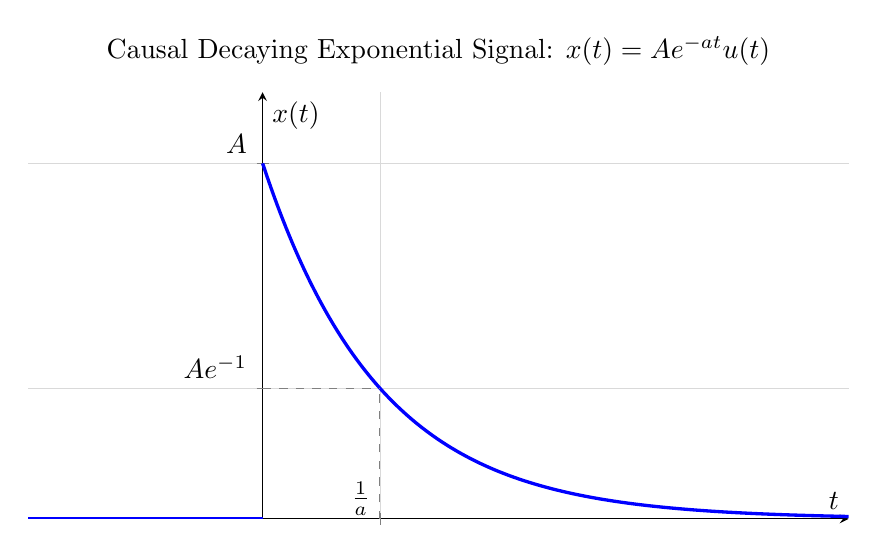
\begin{tikzpicture}
	\begin{axis}[
		width=12cm,
		height=7cm,
		xlabel={$t$},
		ylabel={$x(t)$},
		title={Causal Decaying Exponential Signal: $x(t) = A e^{-at} u(t)$},
		xmin=-2, xmax=5, % Increased xmin to show more of t<0
		ymin=0, ymax=1.2,
		axis lines=middle,
		xtick=\empty,
		ytick=\empty,
		extra x ticks={1},
		extra x tick labels={$\frac{1}{a}$},
		extra y ticks={0.3678, 1},
		extra y tick labels={$Ae^{-1}$, $A$},
		extra tick style={
			ticklabel style={anchor=south east}
		},
		grid=both,
		grid style={line width=.1pt, draw=gray!30},
		samples=200,
		no marks,
		]
		
		% Explicitly draw the zero line for t < 0
		\draw[blue, very thick] (axis cs:-2,0) -- (axis cs:0,0);
		
		% Plot the exponential function for t >= 0
		% The domain is set from 0 to xmax
		\addplot[blue, very thick, domain=0:5] {exp(-x)};
		
		% Add dashed lines to highlight the point at the time constant
		\draw[dashed, gray] (axis cs:1,0) -- (axis cs:1, {exp(-1)});
		\draw[dashed, gray] (axis cs:0,{exp(-1)}) -- (axis cs:1,{exp(-1)});
		
		
	\end{axis}
\end{tikzpicture}
    \caption{The signal $x(t)$ is a causal decaying exponential that starts at a value of $A$ at $t=0$ and decays towards zero as $t \to \infty$.}
    \label{fig:signal}
\end{figure}

\textbf{Solution:}
		
		\textbf{Total Energy:}
		\[ % CORRECTION: Replaced $$ with \[
		E = \int_{0}^{\infty} |x(t)|^2 dt = \int_{0}^{\infty} A^2 e^{-2at} dt = A^2 \left[ \frac{e^{-2at}}{-2a} \right]_{0}^{\infty} = \frac{A^2}{2a}
		\] % CORRECTION: Replaced $$ with \]
		
		\textbf{Average Power (Improved Clarity):}
		\[ % CORRECTION: Replaced $$ with \[ and clarified formula
		P_{av} = \lim_{T \to \infty} \frac{1}{2T} \int_{-T}^{T} |x(t)|^2 dt = \lim_{T \to \infty} \frac{1}{2T} \int_{0}^{T} A^2 e^{-2at} dt = \lim_{T \to \infty} \frac{A^2}{2T} \left( \frac{1 - e^{-2aT}}{2a} \right) = 0
		\] % CORRECTION: Replaced $$ with \]
		
		\textbf{Answer:} $E = \frac{A^2}{2a}$, $P_{av} = 0$
\end{example}

	\vspace{0.5em}
	\hrule
	\vspace{0.5em}
	
	\begin{example}[2. Average Power of Complex Exponential and Sinusoidal Signals]
\textbf{Problem:}
		Determine the average power of:
\begin{enumerate}
    \item $x_1(t) = A e^{j(\omega_0 t + \theta)}$
    \item $x_2(t) = A \cos(\omega_0 t + \theta)$
\end{enumerate}

\textbf{Solution:}
		
		% CORRECTION: Used |A|^2 for rigor
		\textbf{Part 1:} $|x_1(t)|^2 = |A e^{j(\omega_0 t + \theta)}|^2 = |A|^2$. The average power is constant, so $P_{av,1} = |A|^2$.
		
		\textbf{Part 2:} $|x_2(t)|^2 = A^2 \cos^2(\omega_0 t + \theta) = \frac{A^2}{2}(1 + \cos(2\omega_0 t + 2\theta))$
		\[ % CORRECTION: Replaced $$ with \[
		P_{av,2} = \frac{1}{T_0} \int_{0}^{T_0} \frac{A^2}{2}(1 + \cos(2\omega_0 t + 2\theta)) dt = \frac{A^2}{2}
		\] % CORRECTION: Replaced $$ with \]
		
		\textbf{Answer:} $P_{av,1} = |A|^2$, $P_{av,2} = \frac{A^2}{2}$
\end{example}

	\vspace{0.5em}
	\hrule
	\vspace{0.5em}
	
	\begin{example}[3. Time-Shifting of Continuous and Discrete-Time Signals]
\textbf{Problem:}
		Given signals:
		% CORRECTION: Used \\ for line breaks
		\begin{align}
			x(t) &= \begin{cases} A(t-1) & \text{for } 1 \le t \le 2 \\ 0 & \text{otherwise} \end{cases} \\
			x[n] &= \delta[n-1] + \delta[n-2] - \delta[n-3]
		\end{align}
		
		Find: $y_{adv}(t) = x(t+1)$, $y_{del}(t) = x(t-1)$, $y_{adv}[n] = x[n+1]$, $y_{del}[n] = x[n-1]$.
		
		% CORRECTION: Used subfigure environment for proper sub-captions
\begin{figure}[H]
    \centering
			\begin{subfigure}{0.45\textwidth}
        \centering
        \resizebox{!}{5cm}{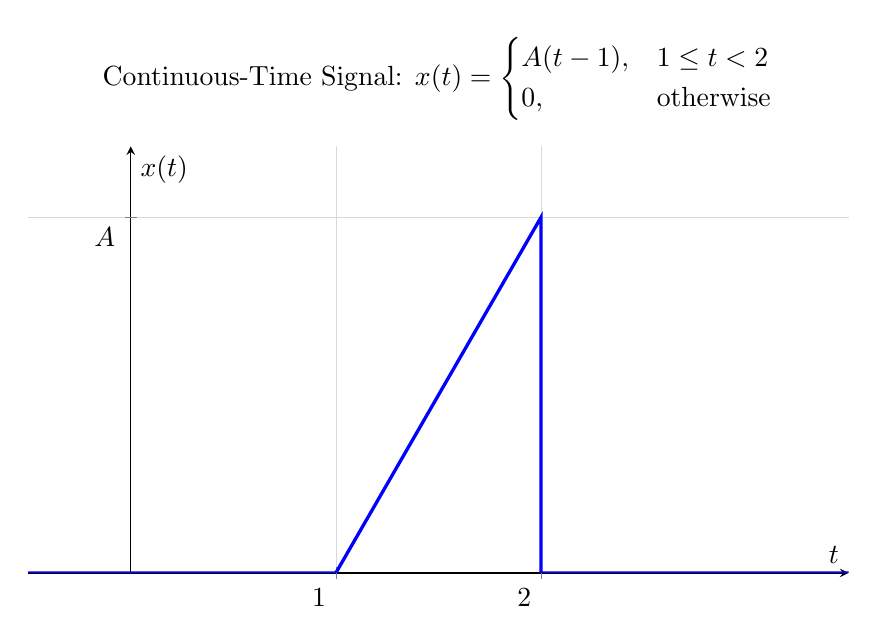
\begin{tikzpicture}
	\begin{axis}[
		% Set the overall style
		width=12cm,
		height=7cm,
		% Axis labels
		xlabel={$t$},
		ylabel={$x(t)$},
		% Title with the formal definition
		title={Continuous-Time Signal: $x(t) = 
			\begin{cases} 
				A(t-1), & 1 \le t < 2 \\ 
				0, & \text{otherwise} 
			\end{cases}$
		},
		% Set axis limits
		xmin=-0.5, xmax=3.5,
		ymin=0, ymax=1.2,
		% Position axes at the origin
		axis lines=middle,
		% Disable default ticks to add custom ones
		xtick=\empty,
		ytick=\empty,
		% Add custom tick marks and labels at key points
		extra x ticks={1, 2},
		extra y ticks={1},
		extra y tick labels={$A$},
		% Style the custom ticks
		extra tick style={ticklabel style={anchor=north east}},
		% Add a grid
		grid=major,
		grid style={line width=.1pt, draw=gray!30},
		]
		
		% Draw the signal shape using axis coordinates for precision
		% This single command creates the sharp edge at t=2
		\draw[blue, very thick]
		(axis cs:-0.5, 0) -- (axis cs:1, 0)   % Zero before t=1
		-- (axis cs:2, 1)                     % Ramp up from t=1 to t=2
		-- (axis cs:2, 0)                     % Discontinuous drop to zero at t=2
		-- (axis cs:3.5, 0);                  % Zero after t=2
		
	\end{axis}
\end{tikzpicture}}
        \caption{The original CT signal $x(t)$.}
			\end{subfigure}\hfill
			\begin{subfigure}{0.45\textwidth}
        \centering
        	\resizebox{!}{5cm}{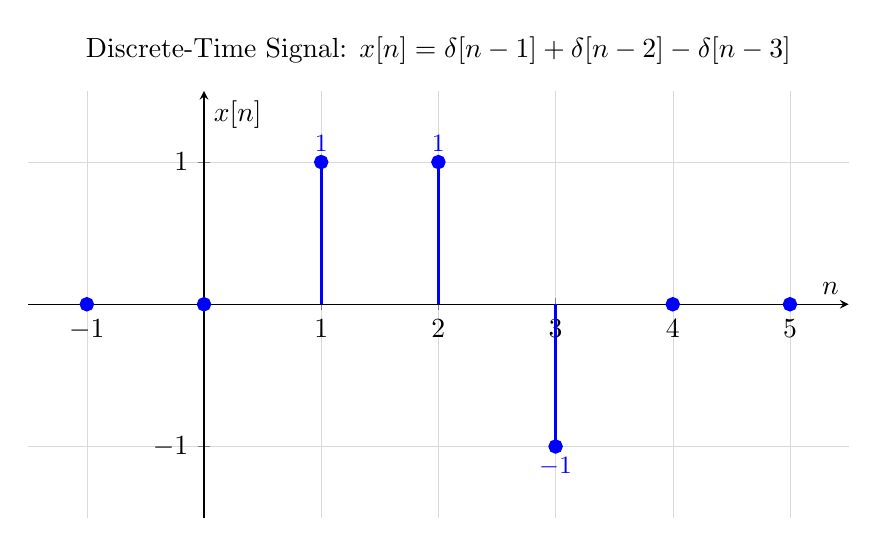
\begin{tikzpicture}
	% Define a style for our stem plots
	\pgfplotsset{
		impulse/.style={
			ycomb,          % Use the 'ycomb' style for stems
			blue,           % Ensure stems and markers are blue
			very thick,     % Thickness of the stems
			mark=*,         % Marker style at the tip of the stem
			mark size=2pt,  % Size of the marker
			draw=blue,      % Ensure the drawing color is blue
			fill=blue,      % Ensure the marker fill is blue
		}
	}
	
	\begin{axis}[
		width=12cm,
		height=7cm,
		title={Discrete-Time Signal: $x[n] = \delta[n-1] + \delta[n-2] - \delta[n-3]$},
		xlabel={$n$},
		ylabel={$x[n]$},
		axis lines=middle,
		xmin=-1.5, xmax=5.5,
		ymin=-1.5, ymax=1.5,
		xtick={-1,0,...,5},
		ytick={-1, 1},
		grid=major,
		grid style={line width=.1pt, draw=gray!30},
		]
		
		% Plot the positive impulses with labels above
		\addplot[
		impulse,
		nodes near coords, % Add value labels
		every node near coord/.style={anchor=south, font=\small}, % Labels above
		] coordinates {
			(1, 1)
			(2, 1)
		};
		
		% Plot the negative impulses with labels below
		\addplot[
		impulse,
		nodes near coords, % Add value labels
		every node near coord/.style={anchor=north, font=\small}, % Labels below
		] coordinates {
			(3, -1)
		};
		
		% Plot the zero-value points (no labels needed)
		\addplot[impulse] coordinates {
			(-1, 0)
			(0, 0)
			(4, 0)
			(5, 0)
		};
		
	\end{axis}
\end{tikzpicture}}
        \caption{The original DT signal $x[n]$.}
			\end{subfigure}
			\caption{The original signals for time-shifting.}
\end{figure}

\textbf{Solution:}
		
		% CORRECTION: Used \\ for line breaks and unique variable names
		\textbf{CT Signal Shifting:}
		\begin{align}
			y_{del}(t) = x(t-1) &= \begin{cases} A(t-2) & \text{for } 2 \le t \le 3 \\ 0 & \text{otherwise} \end{cases} \\
			y_{adv}(t) = x(t+1) &= \begin{cases} At & \text{for } 0 \le t \le 1 \\ 0 & \text{otherwise} \end{cases}
		\end{align}
		
		\textbf{DT Signal Shifting:}
		\begin{align}
			y_{del}[n] = x[n-1] &= \delta[n-2] + \delta[n-3] - \delta[n-4] \\
			y_{adv}[n] = x[n+1] &= \delta[n] + \delta[n-1] - \delta[n-2]
		\end{align}
		% Figures for the solution would also be corrected using the subfigure environment
\end{example}

	\vspace{0.5em}
	\hrule
	\vspace{0.5em}
	
	\begin{example}[4. Combined Time-Scaling and Time-Shifting]
\textbf{Problem:}
		Given:
\[
x(t) = \begin{cases} 
1 & \text{for } -1 < t < 0 \\
1 - 0.5t & \text{for } 0 \le t < 2 \\
0 & \text{otherwise} 
\end{cases}
\]
		
		Find $y(t) = x(-3t - 4)$.

\begin{figure}[H]
    \centering
    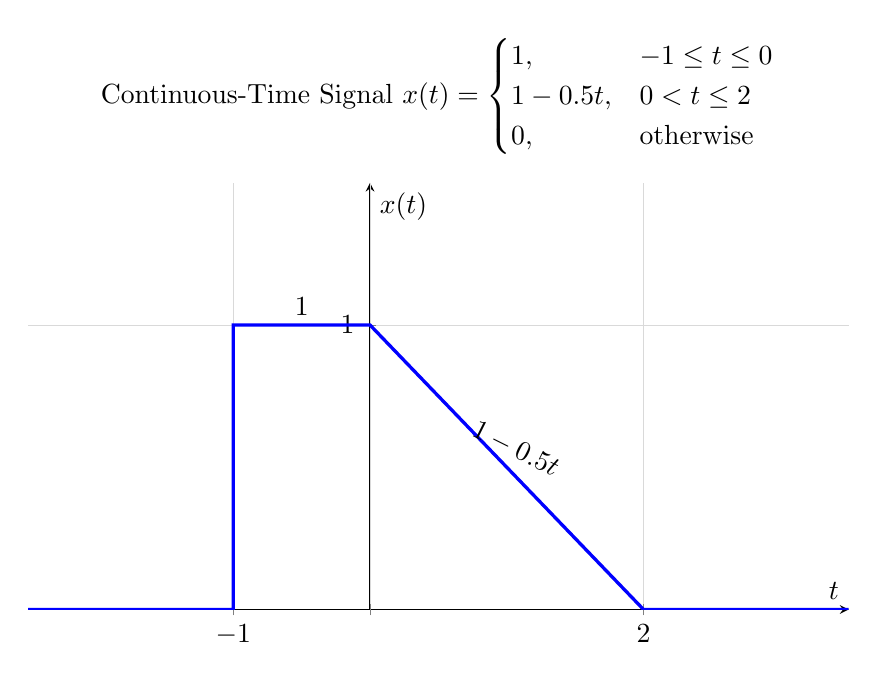
\begin{tikzpicture}
	\begin{axis}[
		% Set the overall style
		width=12cm,
		height=7cm,
		% Title with the formal piecewise definition
		title={Continuous-Time Signal $x(t) = 
			\begin{cases} 
				1, & -1 \le t \le 0 \\
				1 - 0.5t, & 0 < t \le 2 \\
				0, & \text{otherwise} 
			\end{cases}$
		},
		% Axis labels
		xlabel={$t$},
		ylabel={$x(t)$},
		% Position axes at the origin
		axis lines=middle,
		% Set axis limits for good spacing
		xmin=-2.5, xmax=3.5,
		ymin=0, ymax=1.5,
		% Disable default ticks to add custom ones at key points
		xtick=\empty,
		ytick=\empty,
		% --- CORRECTED PART ---
		% Add ticks at key points
		extra x ticks={-1, 0, 2},
		% Provide labels, leaving the label for '0' empty
		extra x tick labels={$-1$,, $2$},
		extra y ticks={1},
		% --- END CORRECTION ---
		% Add a grid
		grid=major,
		grid style={line width=.1pt, draw=gray!30},
		]
		
		% Draw the entire signal shape using axis coordinates for precision
		\draw[blue, very thick]
		(axis cs:-2.5, 0) -- (axis cs:-1, 0) % Zero before t=-1
		-- (axis cs:-1, 1)                   % Vertical jump at t=-1
		-- (axis cs:0, 1)                    % Constant value of 1
		-- (axis cs:2, 0)                    % Ramp down to zero
		-- (axis cs:3.5, 0);                 % Zero after t=2
		
		% Add labels for the function segments
		\node[above] at (axis cs:-0.5, 1) {$1$};
		\node[above, rotate=-26.5] at (axis cs:1, 0.5) {$1 - 0.5t$};
		
	\end{axis}
\end{tikzpicture}
    \caption{The original CT signal $x(t)$.}
    \label{fig:original_signal}
\end{figure}

\textbf{Solution:}
		
		\subsection*{Method 1: Algebraic Substitution (Most Reliable)}
		Substituting $\tau = -3t - 4$:
		\textbf{Interval 1:} $-1 < \tau < 0 \implies -1 < -3t - 4 < 0 \implies -\frac{4}{3} < t < -1$, where $y(t) = 1$.
		\textbf{Interval 2:} $0 \le \tau < 2 \implies 0 \le -3t - 4 < 2 \implies -2 < t \le -\frac{4}{3}$, where $y(t) = 1 - 0.5(-3t - 4) = 3 + 1.5t$.
		
		\subsection*{Method 2: Graphical Step-by-Step (Correct Order)}
		For the general form $y(t) = x(at + b)$, it's crucial to factor the expression inside the parentheses to isolate the time shift:
		\[
		y(t) = x(-3t - 4) = x(-3(t + \frac{4}{3}))
		\]
		
		This form clearly shows the sequence of operations: **SCALE FIRST, THEN SHIFT**.
		
		\textbf{Step 1: Time Scaling and Reversal}
		Start with $x(t)$ and apply the scaling factor $-3$. This involves:
		\begin{enumerate}
			\item \textbf{Scaling:} Compress the signal by a factor of 3 (replace $t$ with $3t$)
			\item \textbf{Reversal:} Reflect the signal about the vertical axis (replace $t$ with $-t$)
		\end{enumerate}
		This gives us the intermediate signal $v(t) = x(-3t)$.
		
		\begin{figure}[H]
			\centering
			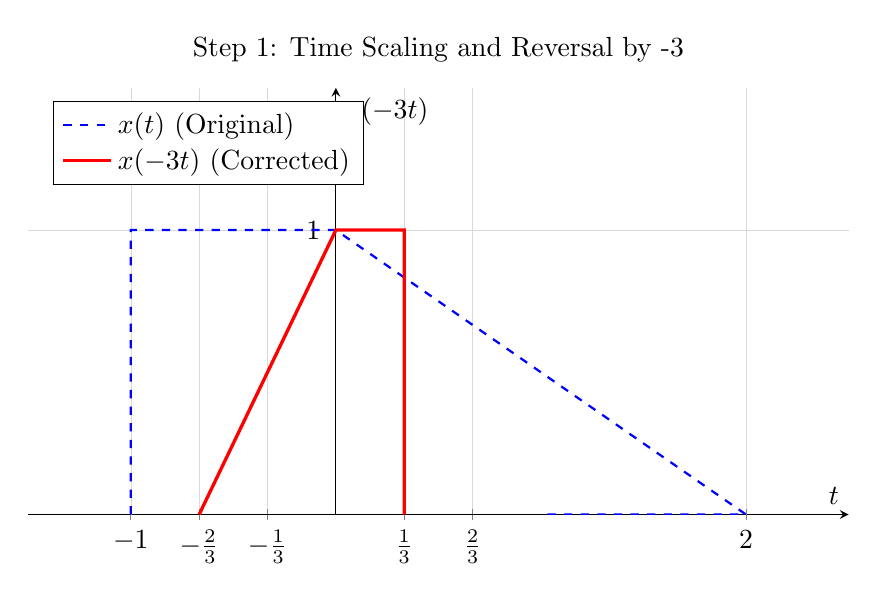
\begin{tikzpicture}
	\begin{axis}[
		% Set the overall style
		width=12cm,
		height=7cm,
		% Title and labels
		title={Step 1: Time Scaling and Reversal by -3},
		xlabel={$t$},
		ylabel={$x(-3t)$},
		% Position axes at the origin
		axis lines=middle,
		% Set axis limits for good spacing
		xmin=-1.5, xmax=2.5,
		ymin=0, ymax=1.5,
		% Set ticks at key fractional and integer points
		xtick={-2/3, -1/3, 0, 1/3, 2/3},
		% Use LaTeX to display tick labels as fractions
		xticklabels={$-\frac{2}{3}$, $-\frac{1}{3}$, $0$, $\frac{1}{3}$, $\frac{2}{3}$},
		ytick={1},
		% --- ADDED LINE ---
		% Add ticks for the original signal's key points
		extra x ticks={-1, 2},
		% --- END ADDED LINE ---
		% Add a grid
		grid=major,
		grid style={line width=.1pt, draw=gray!30},
		% Position the legend
		legend pos=north west,
		legend cell align={left},
		]
		
		% Plot the original signal (dashed blue)
		\addplot[blue, dashed, thick] coordinates {
			(-1,0) (-1,0) (-1,1) (0,1) (2,0) (1,0)
		};
		\addlegendentry{$x(t)$ (Original)};
		
		% Plot the CORRECT scaled and reversed signal (solid red)
		\addplot[red, very thick] coordinates {
			(-2/3, 0) (0, 1) (1/3, 1) (1/3, 0)
		};
		\addlegendentry{$x(-3t)$ (Corrected)};
	\end{axis}
\end{tikzpicture}
			\caption{Step 1: Time scaling and reversal $x(-3t)$ - compress by 3 and reflect.}
			\label{fig:step1_scaling}
		\end{figure}
		
		\textbf{Step 2: Time Shift}
		Now shift the intermediate signal $v(t) = x(-3t)$ left by $\frac{4}{3}$ units to get:
		\[
		y(t) = v(t + \frac{4}{3}) = x(-3(t + \frac{4}{3})) = x(-3t - 4)
		\]
		
		\begin{figure}[H]
			\centering
			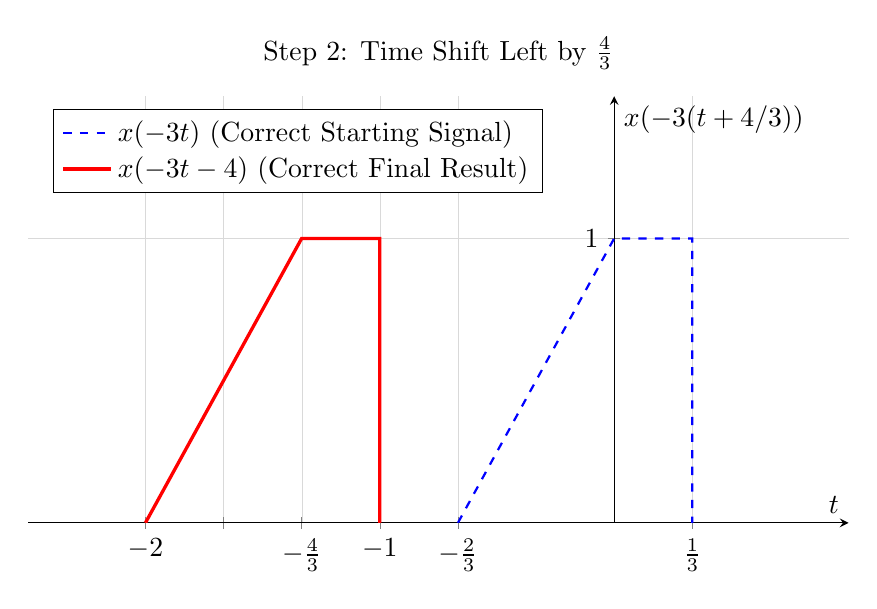
\begin{tikzpicture}
	\begin{axis}[
		% Set the overall style
		width=12cm,
		height=7cm,
		% Title and labels
		title={Step 2: Time Shift Left by $\frac{4}{3}$},
		xlabel={$t$},
		ylabel={$x(-3(t+4/3))$},
		% Position axes at the origin
		axis lines=middle,
		% Set axis limits for good spacing
		xmin=-2.5, xmax=1,
		ymin=0, ymax=1.5,
		% Set ticks at key fractional and integer points
		xtick={-2, -5/3, -4/3, -1, -2/3, 0, 1/3},
		xticklabels={$-2$,,$-\frac{4}{3}$,$-1$,$-\frac{2}{3}$,$0$,$\frac{1}{3}$},
		ytick={1},
		grid=major,
		grid style={line width=.1pt, draw=gray!30},
		legend pos=north west,
		legend cell align={left},
		]
		
		% Plot the CORRECT x(-3t) signal (dashed blue)
		\addplot[blue, dashed, thick] coordinates {
			(-2/3, 0) (0, 1) (1/3, 1) (1/3, 0)
		};
		\addlegendentry{$x(-3t)$ (Correct Starting Signal)};
		
		% Plot the CORRECT shifted signal (solid red)
		% This is x(-3t) shifted left by 4/3
		\addplot[red, very thick] coordinates {
			(-2, 0) (-4/3, 1) (-1, 1) (-1, 0)
		};
		\addlegendentry{$x(-3t - 4)$ (Correct Final Result)};
		
	\end{axis}
\end{tikzpicture}
			\caption{Step 2: Time shift left by $\frac{4}{3}$ to get final result $x(-3t - 4)$.}
			\label{fig:step2_shift}
		\end{figure}
		
		\subsection*{Common Mistakes in Graphical Method}
		Many students make these errors:
		\begin{itemize}
			\item \textbf{Wrong Order:} Applying shift before scaling, which gives incorrect results
			\item \textbf{Incorrect Factoring:} Not properly factoring $x(at + b)$ as $x(a(t + \frac{b}{a}))$
			\item \textbf{Sign Confusion:} Confusing left shift vs. right shift when dealing with negative coefficients
			\item \textbf{Incorrect Intermediate Steps:} Not creating the proper intermediate signal $v(t) = x(at)$ before shifting
		\end{itemize}
		
		\subsection*{Verification}
		Both methods should yield the same result:
\[
y(t) = \begin{cases} 
1 & \text{for } -\frac{4}{3} < t < -1 \\
3 + 1.5t & \text{for } -2 < t \le -\frac{4}{3} \\
0 & \text{otherwise} 
\end{cases}
\]

\begin{figure}[H]
    \centering
    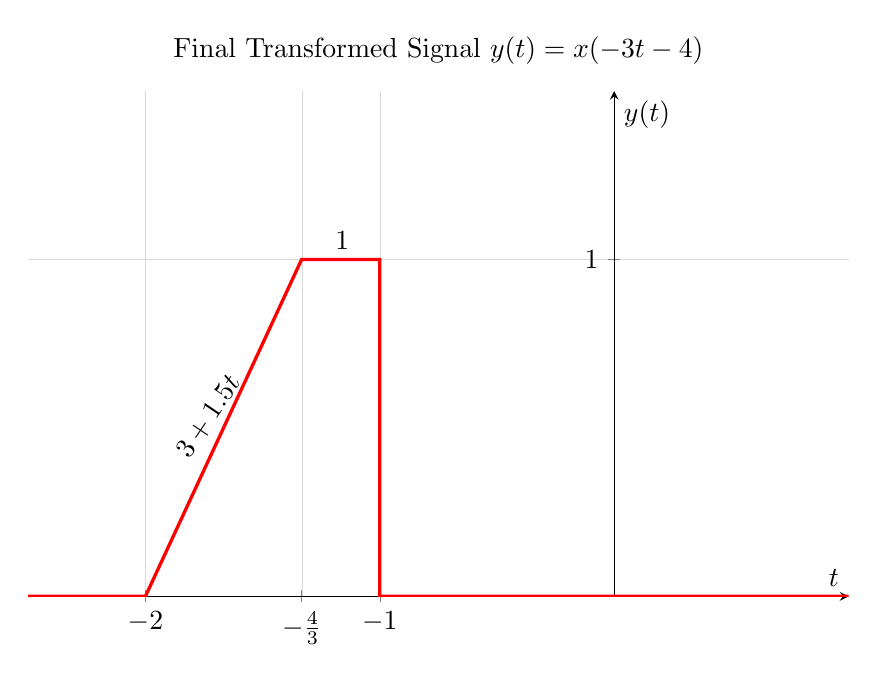
\begin{tikzpicture}
	\begin{axis}[
		% Set the overall style
		width=12cm,
		height=8cm,
		% Title with the final function
		title={Final Transformed Signal $y(t) = x(-3t - 4)$},
		% Axis labels
		xlabel={$t$},
		ylabel={$y(t)$},
		% Position axes at the origin
		axis lines=middle,
		% Set axis limits for good spacing
		xmin=-2.5, xmax=1,
		ymin=0, ymax=1.5,
		% Set ticks at key points
		xtick={-2, -1.333, -1},
		% Use LaTeX to display tick labels as fractions
		xticklabels={$-2$, $-\frac{4}{3}$, $-1$},
		ytick={1},
		% Add a grid
		grid=major,
		grid style={line width=.1pt, draw=gray!30},
		]
		
		% Draw the correct shape of the transformed signal
		\draw[red, very thick]
		(axis cs:-2.5, 0) -- (axis cs:-2, 0)     % Zero before t=-2
		-- (axis cs:-4/3, 1)                     % Ramp up from t=-2 to t=-4/3
		-- (axis cs:-1, 1)                      % Constant value until t=-1
		-- (axis cs:-1, 0)                      % Vertical drop to zero
		-- (axis cs:1, 0);                      % Zero after t=-1
		
		% Add labels for the function segments
		\node[above, rotate=56] at (axis cs:-1.66, 0.5) {$3+1.5t$};
		\node[above] at (axis cs:-1.16, 1) {$1$};
		
	\end{axis}
\end{tikzpicture}
			\caption{The final transformed signal $y(t) = x(-3t - 4)$ obtained by both methods.}
    \label{fig:transformed_signal}
\end{figure}
		
		\subsection*{Key Takeaway}
		For combined transformations $x(at + b)$:
		\begin{enumerate}
			\item \textbf{Always factor first:} $x(at + b) = x(a(t + \frac{b}{a}))$
			\item \textbf{Apply scaling/reversal first:} Create intermediate signal $v(t) = x(at)$
			\item \textbf{Then apply shift:} $y(t) = v(t + \frac{b}{a}) = x(a(t + \frac{b}{a}))$
		\end{enumerate}
		The algebraic substitution method is more reliable and less prone to errors than the graphical method.
\end{example}

\end{document}